% ============================================================
%  BrineWatch — Prototypes for Humanity 2026 application PDF
%  DRAFT — compile: pdflatex BrineWatch_PFH2026_Submission_Draft.tex (x2)
%  All figures are genuine artifacts generated by the code in this
%  repository (official HoloOcean simulator output or matplotlib renders
%  of real run data). No stock or AI-generated imagery.
% ============================================================
\documentclass[10pt,a4paper]{article}

\usepackage[margin=1.75cm,top=1.5cm,bottom=1.6cm]{geometry}
\usepackage[T1]{fontenc}
\usepackage[utf8]{inputenc}
\usepackage{lmodern}
\usepackage{microtype}
\usepackage{xcolor}
\usepackage{graphicx}
\usepackage{titlesec}
\usepackage{enumitem}
\usepackage{booktabs}
\usepackage{textcomp}
\usepackage[hidelinks]{hyperref}

\definecolor{deepblue}{RGB}{11,74,124}
\definecolor{amber}{RGB}{201,135,27}
\definecolor{okgreen}{RGB}{30,125,59}
\definecolor{warnred}{RGB}{192,57,43}

\titleformat{\section}{\sffamily\bfseries\large\color{deepblue}}{\thesection}{0.55em}{}
\titlespacing*{\section}{0pt}{7pt plus 2pt}{3pt}
\titleformat{\subsection}{\sffamily\bfseries\color{deepblue}}{\thesubsection}{0.5em}{}
\titlespacing*{\subsection}{0pt}{5pt}{2pt}
\setlist{nosep,leftmargin=1.15em}
\setlength{\parindent}{0pt}
\setlength{\parskip}{3.0pt}
\graphicspath{{brinewatch/docs/application/pfh2026/assets/}}

\newcommand{\stagebox}[1]{\colorbox{deepblue!10}{\sffamily\small\textbf{#1}}}
\newcommand{\simlabel}[1]{{\scriptsize\sffamily\color{black!55}[#1]}}

\begin{document}

% ===================== PAGE 1 — PROBLEM & PROTOTYPE ===================== %
\begin{minipage}[b]{0.70\textwidth}
  {\sffamily\bfseries\fontsize{22}{24}\selectfont\color{deepblue} BrineWatch}\\[3pt]
  {\sffamily\large Repeatable, uncertainty-aware screening of desalination
  brine plumes with a low-cost ROV}
\end{minipage}\hfill
\begin{minipage}[b]{0.28\textwidth}\raggedleft
  {\sffamily\small Prototypes for Humanity 2026\\[1pt]
  \stagebox{Current stage: Initial Prototype or Model}}
\end{minipage}

\vspace{3pt}{\color{deepblue}\hrule height 1.1pt}\vspace{4pt}

\section{The problem}
Desalination supplies fresh water to hundreds of millions of people and
returns a dense, salty by-product to the sea. Because brine is heavier than
seawater it sinks and spreads along the seabed as a thin, invisible layer —
exactly where routine monitoring is weakest. Vessel casts sample a handful
of points a few times per year; fixed stations rarely sit in the bottom
layer. Regulators enforce mixing-zone limits that, in practice, nobody can
verify continuously; operators get no feedback; communities that depend on
benthic ecosystems get no evidence. Robotic plume mapping has been shown to
be \emph{possible} in research settings; BrineWatch focuses on making it
\textbf{repeatable, adaptive, uncertainty-aware and affordable} — a retrofit
for a BlueROV2-class mini-ROV that many institutions already own.

\section{The prototype at a glance}
\begin{center}
\sffamily\small
Locate \;$\rightarrow$\; Sense \;$\rightarrow$\; Adapt \;$\rightarrow$\;
Reconstruct \;$\rightarrow$\; Screen\\[2pt]
{\footnotesize sonar contacts $\rightarrow$ near-bed CT samples
$\rightarrow$ boundary-aware planning $\rightarrow$ GP map + uncertainty
$\rightarrow$ CLEAR / REVIEW / POSSIBLE EXCEEDANCE}
\end{center}

\begin{minipage}[t]{0.555\textwidth}
  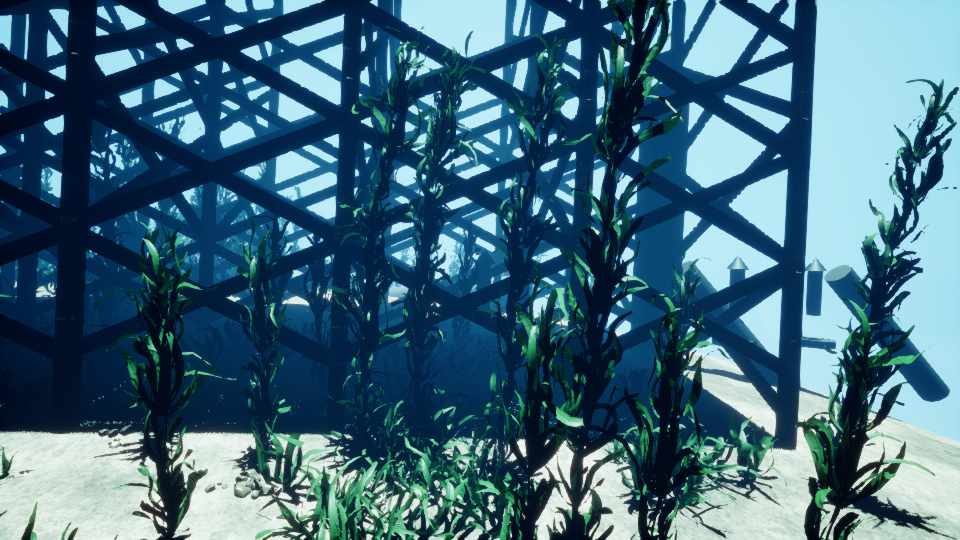
\includegraphics[width=\linewidth]{scene/outfall_side_view.png}\\
  \simlabel{Genuine official-HoloOcean camera frame — the prototype's survey
  site: the outfall hardware (seabed pipe, riser with nozzle) built by the
  terrain-calibrated scene generator at the foot of stock harbor structures.
  The plume is an analytic overlay, never rendered water.}
\end{minipage}\hfill
\begin{minipage}[t]{0.425\textwidth}
  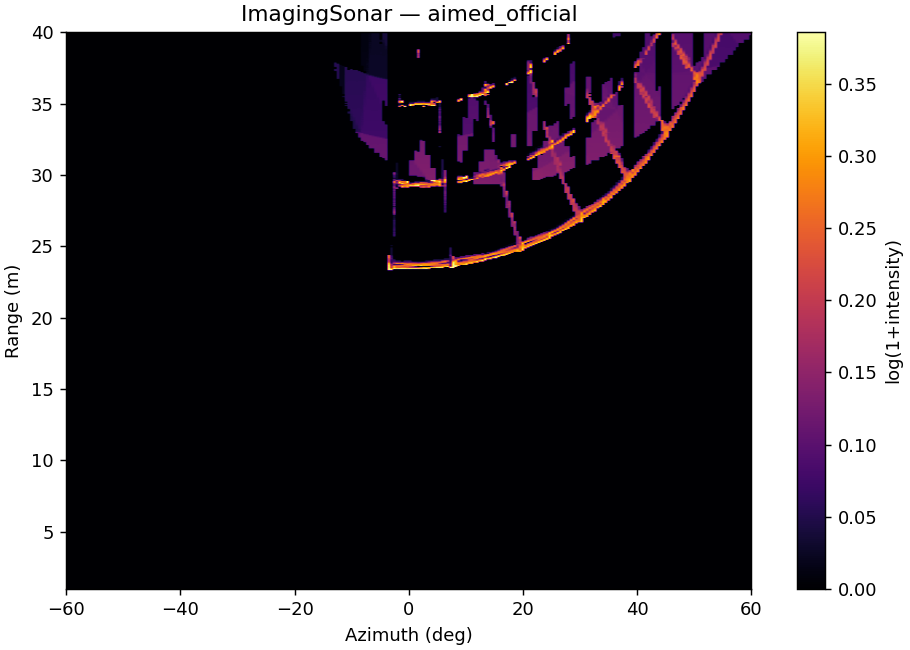
\includegraphics[width=\linewidth]{sonar/pier_sonar_aimed.png}\\
  \simlabel{Genuine official ImagingSonar frame of the same structures:
  bright piling returns with acoustic shadows. The open-water control frame
  is zero everywhere.}
\end{minipage}

\vspace{2pt}
\textbf{What exists today.} A complete autonomous mission stack running
end-to-end in the \emph{official, unmodified} HoloOcean marine simulator
with its stock BlueROV2: sonar-based outfall localization from an
approximate chart position — in the official demonstration mission the
structure was localized with a \textbf{6.4 m error from a 17 m chart prior}
after $\sim$110 m of search, with no access to the true position —
terrain-calibrated navigation over uneven seabed, near-bed
conductivity–temperature sampling of a controlled analytic plume surrogate,
Gaussian-process reconstruction with explicit uncertainty, three-state
screening (correct POSSIBLE-EXCEEDANCE call on the demonstration scenario),
and a self-contained digital mission report. The team owns the
target hardware (BlueROV2 + Omniscan SS450 side-scan sonar); the physical
CT retrofit is specified with a written one-day validation protocol.

% ===================== PAGE 2 — HOW IT WORKS ===================== %
\clearpage
\section{How it works}

\subsection{Official simulator, honest boundaries}
Everything runs on standard HoloOcean 2.3.0 + the official Ocean package —
no engine modifications. Water properties do not exist in the simulator, so
the CT payload samples a documented \emph{analytic surrogate} of a
negatively buoyant discharge (near-field rise and collapse, diluting
bottom-hugging gravity current, tidal advection). The surrogate is not CFD;
its role is to provide exact, seedable ground truth so sampling strategies
and reconstructions can be scored quantitatively.

\subsection{Sonar localization without privileged knowledge}
A controlled experiment proved that runtime-spawned objects are invisible to
the official acoustic pipeline (bit-identical frames with/without them), so
the acoustic target is genuine stock harbor structure and the spawned
outfall geometry is visual dressing — stated as such everywhere. The
detector is classical and reproducible: per-range-row robust background
subtraction, CFAR-like thresholding, component extraction, range/bearing
centroids. Measured on 538 recorded noisy mission frames, single-ping
intensity does \emph{not} separate structure from clutter — so localization
relies on \textbf{spatial persistence}: world-frame contact estimates
accumulated across viewpoints, mode-cluster consensus, aspect-diversity and
chart-plausibility gates. Ground truth is used only by the post-mission
evaluator. Any fallback to the chart prior is loudly flagged in the report
and disqualifies the run as sonar evidence.

\subsection{Boundary-aware adaptive sampling}
After identical LOCATE and BASELINE phases, the survey planner chooses the
next waypoint by a \emph{boundary-aware Gaussian-process acquisition}: a
weighted combination of posterior uncertainty, proximity to the regulatory
isohaline, travel and turning cost (this is a heuristic acquisition, not
formal expected information gain). A fixed lawnmower is kept as the
benchmark baseline and as the routine full-coverage mode.

\subsection{Uncertainty-aware screening, not certification}
The GP posterior yields a near-bed salinity map \emph{and} its uncertainty.
The mission verdict is three-state:
{\color{okgreen}\textbf{CLEAR}} requires both a low worst-case exceedance
probability outside the mixing zone \emph{and} low posterior uncertainty
there — an unsurveyed area can never be declared compliant;
{\color{amber}\textbf{REVIEW}} means the data cannot support a conclusion
(recommended action: re-survey); {\color{warnred}\textbf{POSSIBLE
EXCEEDANCE}} escalates to accredited monitoring. Screening thresholds are
explicit configuration recorded in every report.

\subsection{Implemented vs planned}
\begin{center}\small
\begin{tabular}{@{}p{7.1cm}p{9.2cm}@{}}
\toprule
\textbf{Implemented and exercised (simulation)} & \textbf{Planned (physical transfer)} \\
\midrule
mission autonomy, terrain calibration, sonar pipeline, GP mapping,
screening, digital reports, benchmarks, 86 automated tests &
MAVLink/ArduSub backend (backend swap by design); CT payload retrofit
(BOM specified); Omniscan integration via the same record/replay interface;
one-day controlled water test; harbour trial \\
\bottomrule
\end{tabular}
\end{center}

% ===================== PAGE 3 — VALIDATION ===================== %
\clearpage
\section{Validation evidence}

\subsection{Equal-budget planner benchmark (20 held-out seeds per family)}
\begin{center}
  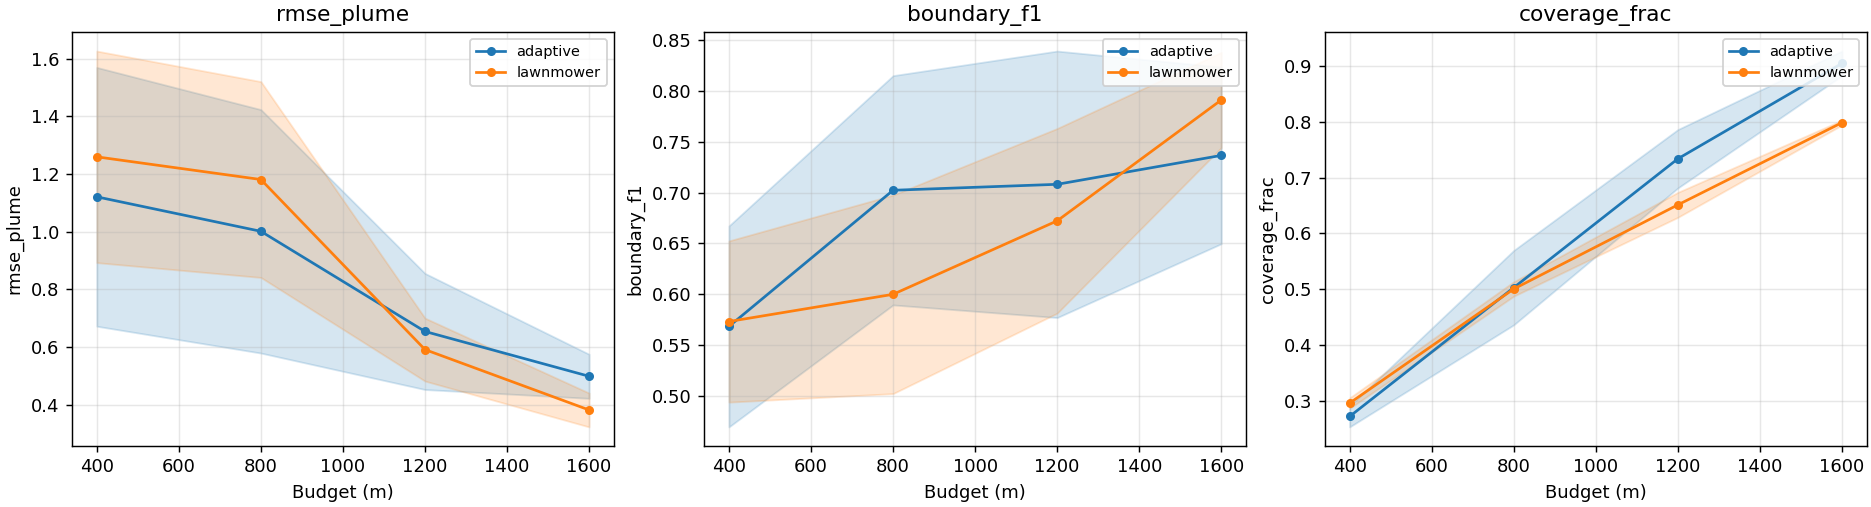
\includegraphics[width=0.98\textwidth]{results/learning_curves_static.png}\\
  \simlabel{Static primary benchmark: reconstruction error, boundary F1 and
  coverage vs travel budget; mean $\pm$ 1$\sigma$ over 20 held-out seeds,
  identical LOCATE/BASELINE, equal budget.}
\end{center}

\begin{minipage}[t]{0.55\textwidth}
\small
\begin{tabular}{@{}lcc@{}}
\toprule
\textbf{Budget} & \textbf{RMSE lawnm.} & \textbf{RMSE adaptive} \\
\midrule
25\,\% & 1.26 $\pm$ 0.37 & \textbf{1.12 $\pm$ 0.45} \\
50\,\% & 1.18 $\pm$ 0.34 & \textbf{1.00 $\pm$ 0.42} \\
75\,\% & \textbf{0.59 $\pm$ 0.11} & 0.65 $\pm$ 0.20 \\
100\,\% & \textbf{0.38 $\pm$ 0.06} & 0.50 $\pm$ 0.08 \\
\bottomrule
\end{tabular}

\vspace{2pt}
{\footnotesize In-plume RMSE (PSU). Boundary F1 at half budget: 0.70
(adaptive) vs 0.60 (lawnmower).}
\end{minipage}\hfill
\begin{minipage}[t]{0.42\textwidth}
\small \textbf{Honest reading.} Adaptive sampling is most useful when the
available survey distance cannot densely cover the area (-11\ldots-15\,\%
RMSE, +17\,\% boundary F1 at 25--50\,\% budget); once the budget saturates
coverage, the lawnmower matches or wins. Across all 320 evaluations of both
families, the three-state screening produced \textbf{zero wrong conclusive
results} — every error of the legacy binary verdict became an honest
REVIEW.
\end{minipage}

\subsection{Sonar evidence and its limits}
\begin{minipage}[t]{0.46\textwidth}
  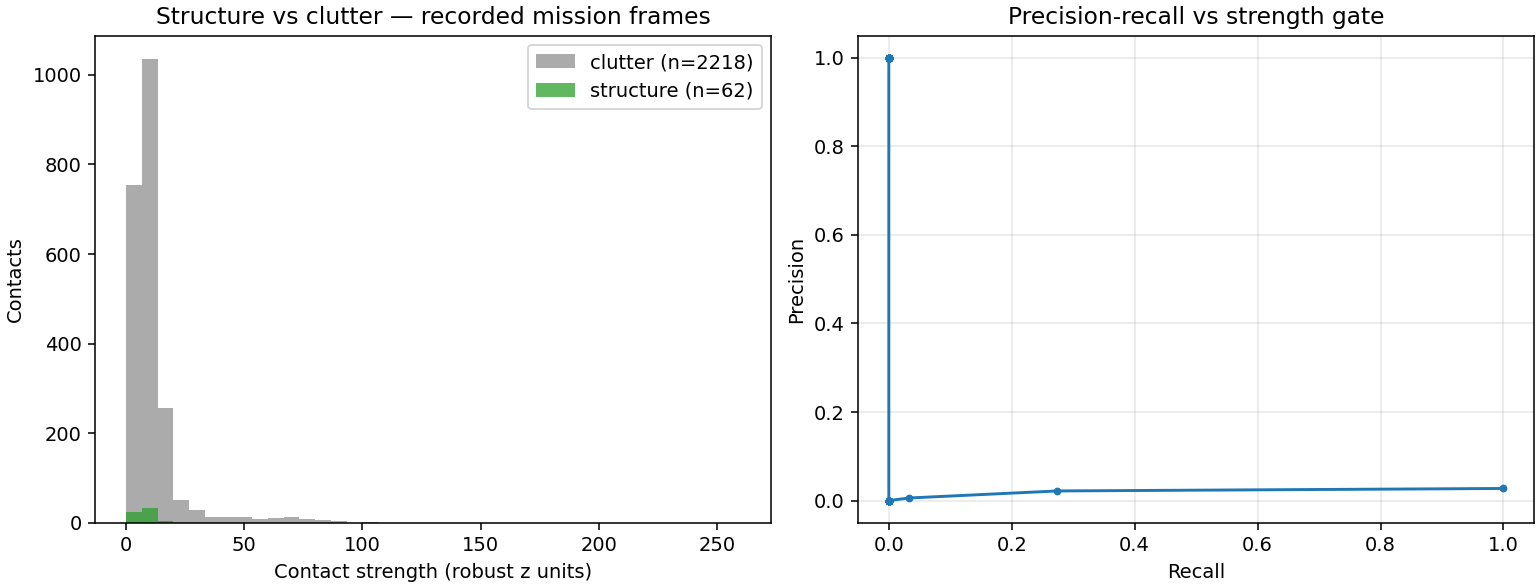
\includegraphics[width=\linewidth]{sonar/detector_eval.png}
\end{minipage}\hfill
\begin{minipage}[t]{0.51\textwidth}
\small Left: on 538 recorded noisy frames, contact-strength distributions
of real structure vs clutter overlap — measured, which is why single-ping
gating was abandoned for persistence-based localization. The
present/absent octree experiment and the open-water zero-control are in the
repository (\texttt{docs/application/pfh2026/assets/sonar/}), together with
the recorded-frame test fixtures that keep the perception suite running
without a simulator.
\end{minipage}

\subsection{The official demonstration mission}
\begin{center}
  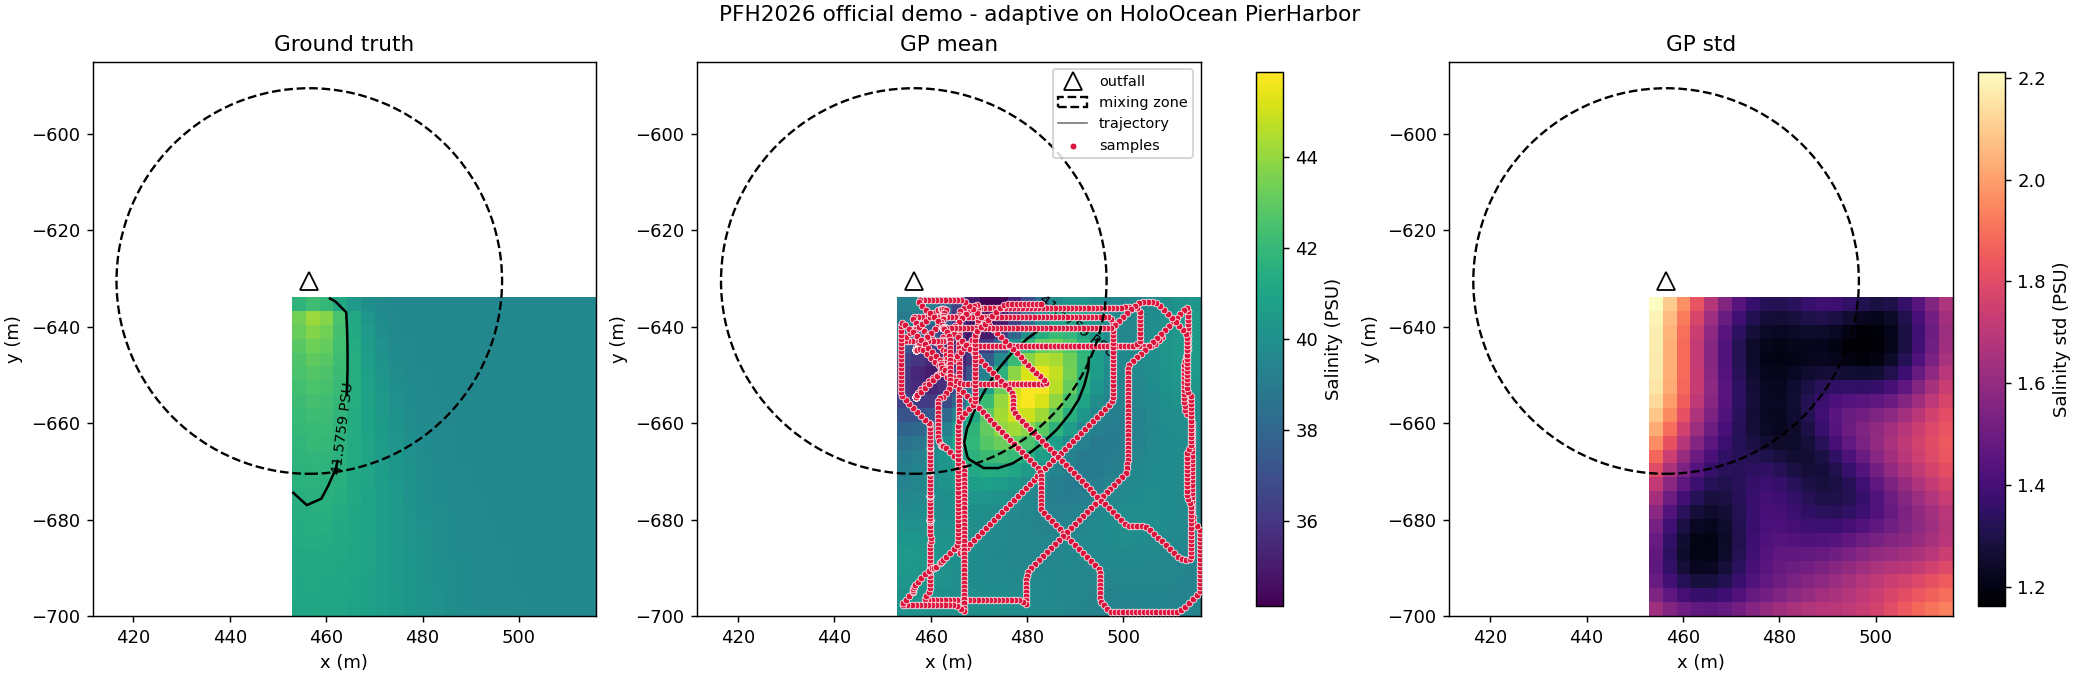
\includegraphics[width=0.98\textwidth]{results/pfh_mission_map.png}\\
  \simlabel{Official HoloOcean mission (PierHarbor, BlueROV2): analytic
  ground truth vs GP reconstruction (trajectory and samples overlaid) vs
  posterior uncertainty. Sonar-confirmed localization error 6.4 m;
  screening: POSSIBLE EXCEEDANCE — correct for this scenario.}
\end{center}

\subsection{Longitudinal screening (simulated campaign)}
\begin{center}
  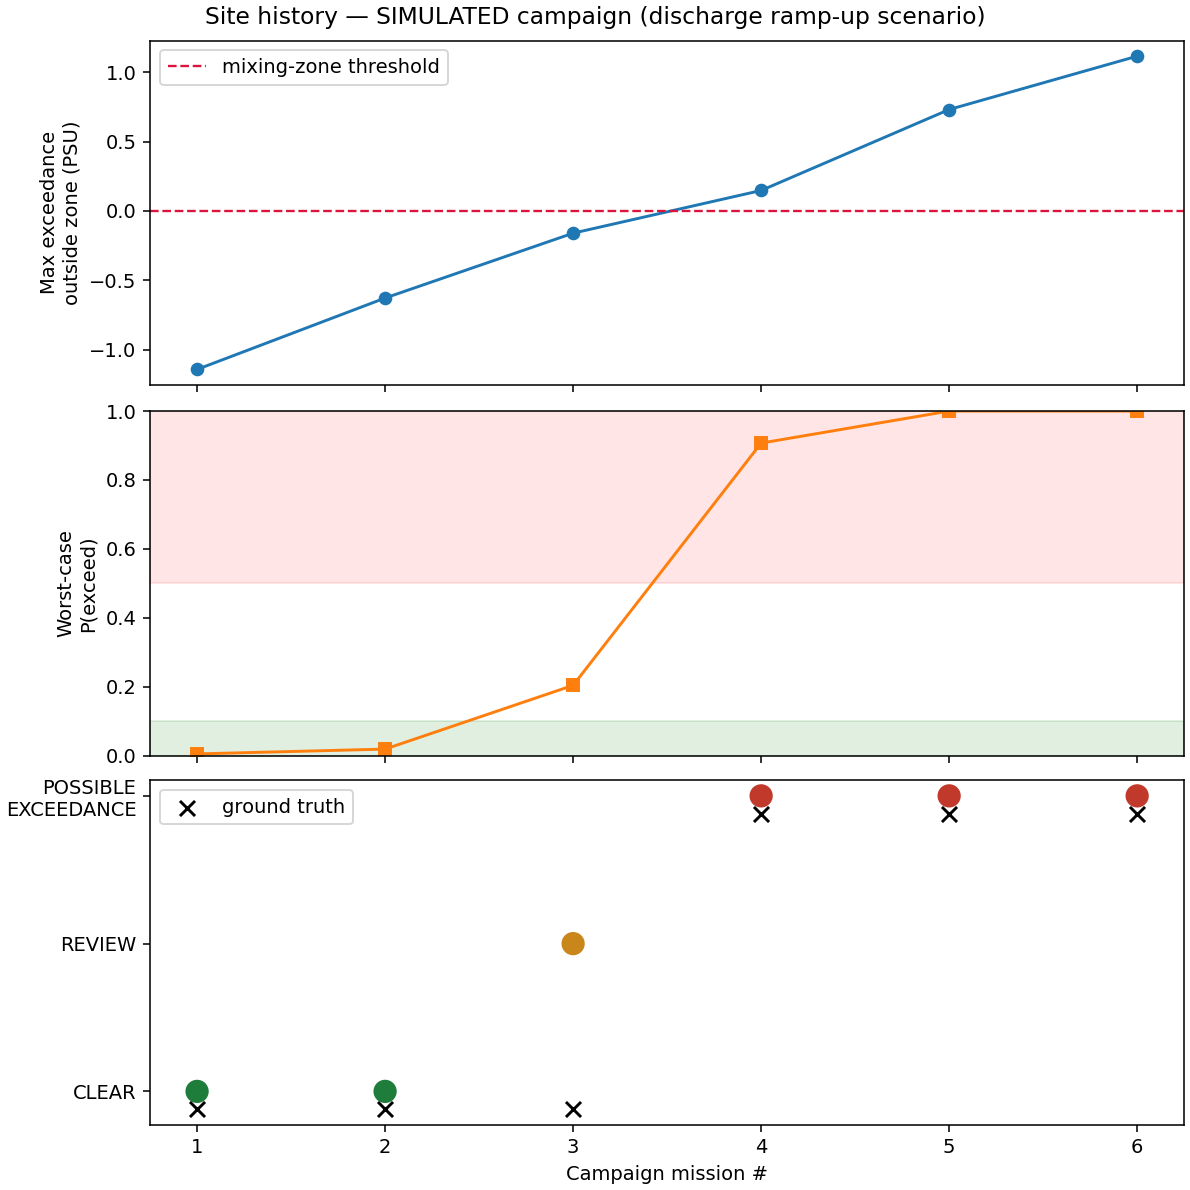
\includegraphics[width=0.9\textwidth]{results/site_history_trend.png}\\
  \simlabel{Six simulated missions over a discharge ramp-up: the screening
  record tracks CLEAR $\rightarrow$ REVIEW $\rightarrow$ POSSIBLE
  EXCEEDANCE, with ground truth marked. Clearly labelled simulated data.}
\end{center}

\textbf{Reproducibility.} \texttt{python -m pytest tests -q} (86 tests, no
GPU needed) \;\textperiodcentered\; \texttt{python scripts/run\_mission.py}
(kinematic demo) \;\textperiodcentered\;
\texttt{python scripts/run\_benchmark.py --seeds 20 --seed-start 100}
\;\textperiodcentered\; \texttt{python scripts/run\_pfh2026\_demo.py}
(official HoloOcean mission). Repository:
\url{https://github.com/AndreaBedei1/DubaiProposal}

% ===================== PAGE 4 — IMPACT & ROADMAP ===================== %
\clearpage
\section{Impact}
\textbf{Who uses it.} Utilities and plant operators (feedback instead of
biannual snapshots), municipalities and environmental regulators
(affordable verification of mixing-zone conditions), and university or NGO
laboratories in desalination-dependent regions — the users who cannot
charter survey vessels routinely. \textbf{Why repeated low-cost surveys
matter.} Brine impact is chronic, not episodic: a single yearly snapshot
cannot separate tides, seasons and plant load. A mini-ROV mission costs a
morning and a battery; the screening record turns repetition into evidence
— and the REVIEW state tells operators exactly when a survey was
insufficient rather than pretending certainty.

\section{Roadmap}
\begin{enumerate}
\item \textbf{Controlled water test (one day, protocol written):} CT probe
  calibration, response-time test, salinity-gradient pool survey, GP map
  vs reference casts — first non-simulated entry in the site history.
\item \textbf{Harbour trial:} a known freshwater inflow as a safe,
  permit-free salinity anomaly; MAVLink backend replaces the simulator
  backend (the mission layer is unchanged by design).
\item \textbf{Real outfall pilot} with a utility or regulator partner:
  site-specific mixing-zone configuration, comparison against accredited
  vessel casts.
\end{enumerate}

\section{Limitations (complete ledger in the repository)}
Analytic plume surrogate, not CFD; virtual water properties; simulated
sonar-to-real-sonar domain gap (thresholds must be re-tuned on real
acoustics); idealized navigation; screening is \emph{not} regulatory
certification; no field validation yet; single vehicle; demo mixing zone
scaled to the simulator world (all radii configurable).

\section{Team}
Andrea Bedei — PhD student, University of Bologna (MSc Automotive
Engineering for Intelligent Mobility, 2025); supervisors Giovanni Pau and
Roberto Girau, University of Bologna. Industrial support: MBS (marine
robotics). Hardware available to the team: BlueROV2, Cerulean Omniscan
SS450.

\vspace{4pt}{\color{deepblue}\hrule height 0.7pt}\vspace{3pt}
{\footnotesize All figures in this document are genuine artifacts of the
public repository: official HoloOcean simulator captures or matplotlib
renders of recorded run data. Simulated content is labelled as such.
BrineWatch is an initial prototype; it does not claim field validation,
certification or commercial readiness.}

\end{document}
